\documentclass{standalone}

% Plotting
\usepackage{tikz}
\usetikzlibrary{decorations.markings}
\usetikzlibrary{calc}
% quantikz breaks tikz-cd, see https://tex.stackexchange.com/questions/618330/quantikz-breaks-spacing-in-tikz-matrices-tikz-cd
%\usetikzlibrary{quantikz}
\usetikzlibrary{cd}
\usepackage{pgfplots}

\usepackage{simpler-wick}
\usepackage{physics}

\usepackage{amsmath}
\usepackage{mathtools}

\begin{document}
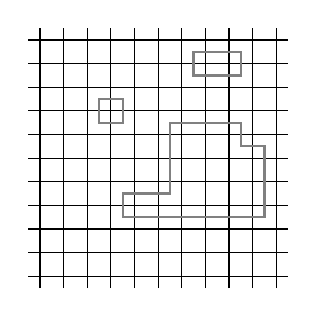
\begin{tikzpicture}[scale=1.5,decoration={
    markings,
    mark=at position 0.5 with {\arrow{>}}}]

    \foreach \i in {0,0.2,...,2} {
        \draw (\i, -0.1) -- (\i, 2.1);
    }

    \foreach \i in {0,0.2,...,2} {
        \draw (-0.1, \i) -- (2.1, \i);
    }

    \draw[thick, gray] (0.5, 1.3) -- ++(0, 0.2) -- ++(0.2, 0) -- ++(0, -0.2) -- cycle;
    \draw[thick, gray] (1.3, 1.7) -- ++(0, 0.2) -- ++(0.4, 0) -- ++(0, -0.2) -- cycle;
    \draw[thick, gray] (0.7, 0.5) -- ++(0, 0.2) -- ++(0.4, 0) -- ++(0, 0.6) -- ++(0.6, 0) -- ++(0, -0.2) --++ (0.2, 0) -- ++(0, -0.6) -- cycle;
\end{tikzpicture}
\end{document}